\section{Type-$(n, 1, 1)$ instances}

\subsection{As a maximum-cost maximum-flow problem}
This restriction is also squarely in \textsc{P}, again shown via a maximum-cost maximum-flow algorithm.

For every course, there's a single weekly schedule it has chosen. Thus we can precompute a function $f(l, h)$, which for every course $l$, returns the day of the $h$th class For presentation purposes, we will define $L_{l, h, k} = (\min(l, h, k), \max(l, h, k))$.

We can construct the following flow network:

\begin{center}
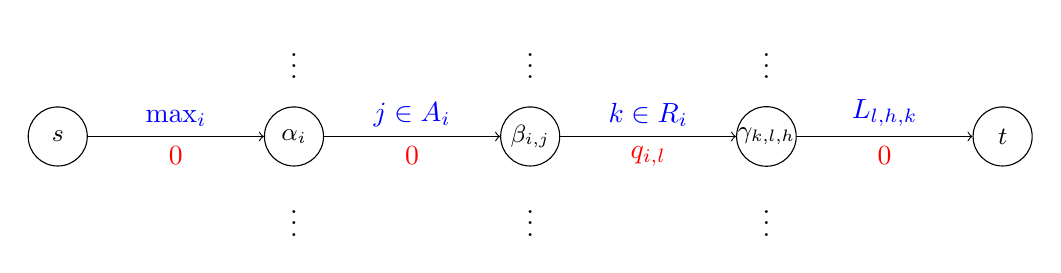
\begin{tikzpicture}

\tikzstyle{v}=[draw, circle, inner sep=0pt, font=\small, align=center, minimum size=0.75cm];
\tikzstyle{e}=[->, dashed];

\node[v] (s) at (1, 1) {$s$};
\node[v] (alpha_i) at (4, 1) {$\alpha_i$};
\node (d1) at (4, 0) {$\vdots$};
\node (d2) at (4, 2) {$\vdots$};
%\node[v] (alpha_1) at (4, 3) {$\alpha_1$};
%\node[v] (alpha_p) at (4, -1) {$\alpha_p$};

\node[v] (beta_ij) at (7, 1) {$\beta_{i, j}$};
\node (d3) at (7, 0) {$\vdots$};
\node (d4) at (7, 2) {$\vdots$};
%\node[v] (beta_11) at (7, 3) {$\beta_{1, 1}$};
%\node[v] (beta_pd) at (7, -1) {$\beta_{p, d}$};

\node[v] (gamma_klj) at (10, 1) {$\gamma_{k, l, h}$};
\node (d5) at (10, 0) {$\vdots$};
\node (d6) at (10, 2) {$\vdots$};

%\node[v] (gamma_111) at (10, 3) {$\gamma_{1, 1, 1}$};
%\node[v] (gamma_mcv) at (10, -1)  {$\gamma_{m, c, v}$};

\node[v] (t) at (13, 1) {$t$};

\draw[->] (s) to node[blue, above] {$\max_i$} node[red, below] {$0$} (alpha_i);

%\dottedarrows{{s}}{{alpha_1, alpha_p}};

\draw[->] (alpha_i) to node[blue, above] {$j \in A_i$} node[red, below] {$0$} (beta_ij);

%\dottedarrows{{alpha_1, alpha_i, alpha_p}}{{beta_11, beta_ij, beta_pd}}{alpha_i}{beta_ij};

\draw[->] (beta_ij) to node[blue, above] {$k \in R_i$} node[red, below] {$q_{i, l}$} (gamma_klj);

%\dottedarrows{{beta_11, beta_pd, beta_ij}}{{gamma_111, gamma_mcv, gamma_klj}}{beta_ij}{gamma_klj};

%\dottedarrows{{gamma_111, gamma_mcv}}{{t}};

\draw[->] (gamma_klj) to node[blue, above] {$L_{l, h, k}$} node[red, below] {$0$} (t);
\end{tikzpicture}
\end{center}

Formally, this is $G = (V, E)$, such that

\begin{align*}
  V = &\{s\} \cup \{t\}\\
      &\cup \{\alpha_i \mid i \in P\}\\
      &\cup \{\beta_{i, j} \mid i \in P, j \in S\}\\
      &\cup \{\gamma_{k, l, h} k \in R, l \in C, 1 \le h \le n(l)\}\\
  E = &\{(s, \alpha_i)\ \forall\ i\}\\
      &\cup \{(\alpha_i, \beta_{i, j}) \ \forall\ i, j \mid j \in A_i\}\\
      &\cup \{(\beta_{i, j}, \gamma_{k, l, h})\ \forall\ i, j, k, l, h \mid k \in R_i, f(l, h) = j\}\\
      &\cup \{(\gamma_{k, l, h}, t) \ \forall\ k, l, h\}
\end{align*}

with capacity function $c:E \to \Z^2$ such that
\begin{align*}
  c(s, \alpha_i) &= (0, \textstyle\max_i)\\
  c(\alpha_i, \beta_{i, j}) &= (0, j \in A_i)\\
  c(\beta_{i, j}, \gamma_{k, l, h}) &= (0, k \in R_i)\\
  c(\gamma_{k, l, h}, t) &= L_{l, h, k} = (\min(l, h, k), \max(l, h, k))
\end{align*}

where a capacity of $(a, b)$ means a lower bound of $a$ and an upper bound of $b$; and weighed by $w:E \to \mathbb{R}$, such that
\begin{align*}
  w(e) = \begin{cases}
    q_{i, l} & \text{ if } e = (\beta_{i, j}, \gamma_{k, l, h})\\
    0 & \text{otherwise}
  \end{cases}
\end{align*}

This solves the problem in a similar way as the single course day. A unit of flow going through $(\alpha_i, \beta_{i, j})$ repersents professor $i$ working on the $j$th day. If this unit flows through $(\beta_{i, j}, \gamma_{k, l, h})$, this represents working as the $k$th role on the $h$th class of the $l$th course.

The constraints on the outgoing flow for $\gamma_{k, l, h}$ imply that the only way to obtain a flow of $\sum_{k, l, h} n_{k, l, h}$ units is that each outgoing edge is saturated. Thus a maximum flow of that magnitude is equivalent to a valid assignment of professors to roles in each class of each course.

Furthermore, we wish to maximize the quality of each professor teaching each course. This means maximizing the sum of the $q_{i, l}$, since this represents that the $i$th professor is teaching a class of the $l$th course. Thus among these maximum flows, we want the one of maximum cost.

Since this problem is solvable in polynomial time in the number of nodes and edges of the network, and in our case these are also in $O(poly(p, d, m, v, c))$, the problem is solvable in polynomial time, and thus is also in \textsc{P}.


\subsection{As a maximum-weight perfect bipartite matching}
Again in the case where professors have no upper bound on the number of classes they can teach, and the role requirements for each class have the same upper and lower bounds, we can view this restriction a maximum-weight perfect matching on a bipartite graph. The construction is similar to the single course case:

\begin{center}
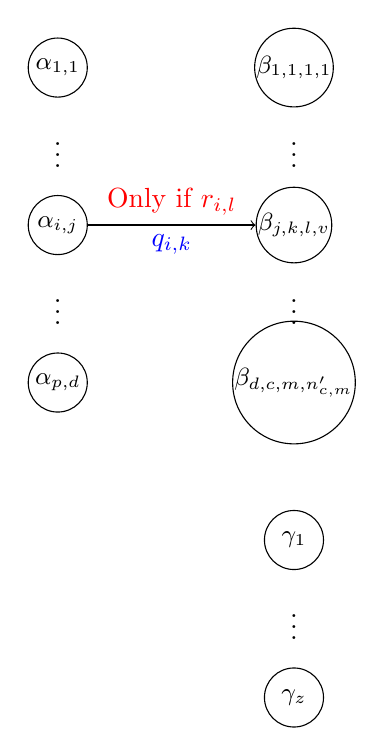
\begin{tikzpicture}
  \node[v] (a11) at (0, 4) {$\alpha_{1, 1}$};
  \node (d1) at (0, 3) {$\vdots$};
  \node[v] (aij) at (0, 2) {$\alpha_{i, j}$};
  \node (d2) at (0, 1) {$\vdots$};
  \node[v] (ant) at (0, 0) {$\alpha_{p, d}$};

  \node[v] (b1111) at (3, 4) {$\beta_{1, 1, 1, 1}$};
  \node (d3) at (3, 3) {$\vdots$};
  \node[v] (bjklv) at (3, 2) {$\beta_{j, k, l, v}$};
  \node (d4) at (3, 1) {$\vdots$};
  \node[v] (btcmncm) at (3, 0) {$\beta_{d, c, m, n'_{c, m}}$};

  \node[v] (c1) at (3, -2) {$\gamma_1$};
  \node (d5) at (3, -3) {$\vdots$};
  \node[v] (cz) at (3, -4) {$\gamma_z$};

  \draw[->] (aij) to node[above, red] {Only if $r_{i, l}$} node[below, blue] {$q_{i, k}$} (bjklv);
  \dottedarrows{{a11, aij, ant}}{{b1111, bjklv, btcmncm, c1, cz}}{aij}{bjklv};
\end{tikzpicture}
\end{center}

Formally, we have a graph $G = (V, E)$, where

\begin{align*}
  V = & \{\alpha_{i, j} \mid 1 \le i \le p, 1 \le j \le d, a_{i, j} = 1\}\\
    & \cup \{\beta_{j, k, l, v} \mid 1 \le j \le d, 1 \le k \le c, 1 \le l \le m, 1 \le v \le n'_{c, l}\}\\
    & \cup \{\gamma_i \mid 1 \le i \le z\}\\
  E = & \{\{\alpha_{i, j}, \beta_{j, k, l, v}\}\ \forall\ i, j, k, l, v, r_{i, l} = 1\}\\
      & \cup \{\{\alpha_{i, j}, \gamma_k\} \mid \ \forall\ i, j, k\}
\end{align*}

where we have defined, as before, $x = \sum_{i = 1}^p |\{j \mid 1 \le j \le d, a_{i, j} = 1\}|$, $y = \sum_{k = 1}^c \sum_{l = 1}^m n'_{k, l}$, and $z = x - y$.

We also have a cost function $w:E \to \mathbb{R}$, such that:

\begin{align*}
  w(\alpha_{i, j}, \beta_{j, k, l, v}) &= q_{i, k}\\
  w(\alpha_{i, j}, \gamma_k) &= 0
\end{align*}

Conceptually, we see this as assigning proffesors $i$, on day $j$, to either teach the $k$th course, on the $l$th role (being the $v$th instance of this role for that class), or to have a ``holiday'', when they're assigned to some $\gamma$. The cost of assigning a professor to teach a class is the quality the professor has for that class, hence what we want to maximize is the sum of the costs of the professor assignments in this bipartite graph.

This formulation again provides us with an integer linear programming formulation, noting by $B$ the incidence matrix of $G$:

\begin{alignat*}{2}
  \text{maximize }   & q^t x \\
  \text{subject to } & Bx \le \mathbf{1}\\
                     & x ge \mathbf{0}\\
                     & x \in \mathbb{Z}^M
\end{alignat*}

which, by unimodularity of $B$ since $G$ is bipartite,  has an integral linear relaxation:

\begin{alignat*}{2}
  \text{maximize }   & q^t x \\
  \text{subject to } & Bx \le \mathbf{1}\\
                     & x \ge \mathbf{0}\\
                     & x \in \mathbb{R}^M\\
\end{alignat*}

and thus an optimal solution can be found in polynomial time in the size of $B$, which by our construction of $G$ is in $O(poly(p, t))$.
